\input{configuration}

\title{Lecture 6 --- Data Definition  }

\author{Jeff Zarnett \\ \small \texttt{jzarnett@uwaterloo.ca}}
\institute{Department of Electrical and Computer Engineering \\
  University of Waterloo}
\date{\today}


\begin{document}

\begin{frame}
  \titlepage

 \end{frame}
 
 
\begin{frame}
\frametitle{Data Definition}

We have thus far not yet learned about how to formally create relations.

The SQL data definition language (DDL) looks a lot like the query language that we have used thus far.

\begin{center}
	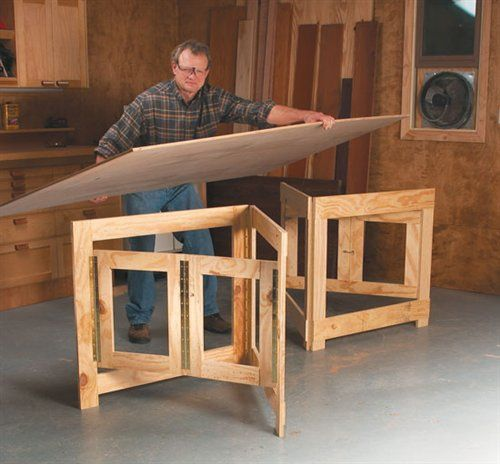
\includegraphics[width=0.4\textwidth]{images/make-table.jpg}
\end{center}

 \end{frame}
 
 
\begin{frame}
\frametitle{Data Definition}


Specifically, our data definition language allows us to define:
\begin{itemize}
	\item The schema of each relation.
	\item The type of each attribute.
	\item Integrity constraints.
	\item Indices on relations.
	\item Security/authorization information for a relation.
	\item Physical storage structure.
\end{itemize}

\end{frame}


\begin{frame}
\frametitle{SQL Standard Types}

Attributes have types; the SQL standard includes the following built-in types:

\begin{itemize}
\item \textbf{char}$(n)$
\item \textbf{varchar}$(n)$
\item \textbf{int} (or \textbf{integer})
\item \textbf{smallint}
\item \textbf{numeric}$(p, d)$
\item \textbf{real}
\item \textbf{double precision}
\item \textbf{float}$(n)$
\item \textbf{boolean}
\item \textbf{date}, \textbf{time}, \textbf{datetime}
\end{itemize}

\end{frame}

\begin{frame}
\frametitle{Creating a Table}

If we wish to define a SQL relation, the syntax for this is to create a relation (table) is called (unsurprisingly), \texttt{CREATE TABLE}. 

The syntax for this command requires a name as well as a listing of the attributes (fields) and their types (definitions). 

It is also customary to include at least one constraint, the primary key. 

As before we put a semicolon at the end of the statement to designate the end of the statement. 

\end{frame}

\begin{frame}[fragile]
\frametitle{Creating a Table}


{\small
\begin{verbatim}
CREATE TABLE r
 (A1 D1, A2 D2, ... An Dn,
 integrity-constraint-1,
 ...
  integrity-constraint-k);
\end{verbatim}
}

A more concrete example: 
{\small
\begin{verbatim}
CREATE TABLE student
 (id varchar(8),
  userid varchar(8) NOT NULL,
  firstname varchar(64),
  lastname varchar(64),
  birthday date,
  department_id int default 0,
  PRIMARY KEY( id ),
  FOREIGN KEY( department_id ) REFERENCES department( id )
 );
\end{verbatim}
}

\end{frame}


\begin{frame}
\frametitle{Attribute Observations}

On some attributes an additional qualifier \texttt{not null} was added. 

This means that a value of \texttt{null} is forbidden from being assigned to that attribute. 

The department ID attribute has a default value.

The primary-key definition in this case specifies that \texttt{id} is the primary key for the relation.

The last sort of constraint that is shown in the example is the foreign key constraint that mentions the department ID.

\end{frame}

\begin{frame}
\frametitle{Foreign Key Behaviour}

It is not shown in the diagram but we can override the default behaviour for what happens if the foreign key constraint is violated. 

\begin{center}
	
\includegraphics[width=0.5\textwidth]{images/breaking-the-law.jpg}
\end{center}

\end{frame}

\begin{frame}
\frametitle{Foreign Key Behaviour}

Rather than rejecting the update we could choose if we want:

(1) to cascade the changes, or 

(2) setting null if the value is invalid, or 

(3) setting some default value.

\end{frame}


\begin{frame}
\frametitle{Reject the Heretic}

My personal preference is that we stick with rejection.

It is better to prevent insertion of wrong data (and fix it at the source) rather than let it proceed and cover it up by putting a null in there. 

In the words of my friend Tuomo Jorri: 

If the date calculation is consistently off by 42 days, instead of a statement that says (date = date - 42), you should figure out why the date is off by 42 and fix it.

\end{frame}


\begin{frame}
\frametitle{Unique Constraint}

Not shown in the example above is the \textit{unique} constraint. 

\begin{center}
	
\includegraphics[width=0.3\textwidth]{images/only-one.jpg}
\end{center}

This requires simply that no two tuples of the relation may be equal in a particular attribute. 

Because null is not equal to null in the SQL standard, many tuples may have null for this value.

\end{frame}

\begin{frame}
\frametitle{Check Constraints}

It is possible (although rare, at least in my experience) to also add a \alert{check} clause as a constraint. 

The check clause takes a predicate and any insertion or update is is evaluated to see if it is consistent with this constraint. 

A check that says \texttt{salary > 0} ensures that an employee cannot be put into the database with a negative salary amount. 

A check constraint predicate can be arbitrarily restrictive, allowing business logic to be embedded in the database.

\end{frame}


\begin{frame}
\frametitle{Foreign Keys Can Have Names}

We did not do this in the above case, but we can put a name to foreign keys or other constraints. 

The name must be unique in the database schema. 

We'll look at adding names when we talk about altering tables. 

Names can be useful though, because a well-named constraint can tell you what has gone wrong.

\end{frame}

\begin{frame}
\frametitle{Now, Or Later?}

Another way that adding a foreign key fails? The target relation doesn't exist. 

This means we would have to create relations in some order that means the foreign keys are all satisfied at the time of the creation. 

That might not be realistic, though, based on the desired schema. 

Fortunately, we can add them in later.

\end{frame}


\begin{frame}
\frametitle{Altering Tables}

In addition to adding in some integrity constraints we can change the table definition, or remove constraints. 

\begin{center}
	
\includegraphics[width=0.4\textwidth]{images/alter-deal.jpg}
\end{center}

The command for this is \texttt{ALTER TABLE} and we will need to specify the table to be modified as well as the change that we would like to make. 

\end{frame}

\begin{frame}
\frametitle{Adding a Column}

If we want to add a new column to the table, then the alter table syntax requires us to specify the name of the new attribute to be added and the type. 

\texttt{ALTER TABLE students ADD COLUMN email VARCHAR(128);} 

\end{frame}

\begin{frame}
\frametitle{Adding a Column}


Subsequent to that we can make additional changes, such as adding an index, or putting in a reference constraint.

At the time of creation, we can set a default value and set not-null.

Note that is is possible to add multiple elements in a single statement. 

\end{frame}

\begin{frame}
\frametitle{Dropping a Column}

The mirror operation to that is to drop a column: 

\texttt{ALTER TABLE students DROP COLUMN email;} 

This deletes the attribute from the database and all the data that is in there, \alert{permanently}. 

\begin{center}
	
\includegraphics[width=0.4\textwidth]{images/let-him-go.jpg}
\end{center}
\hfill \textit{``I let him go.''}

\end{frame}

\begin{frame}
\frametitle{Dropping a Column}


Dropping the column can fail if the column is used in a foreign key or other constraint. 

It may also be necessary to remove an index... 

\end{frame}

\begin{frame}
\frametitle{Renaming a Table}

If we wish to rename a table, the keyword we need is \texttt{RENAME}: 

\texttt{ALTER TABLE students RENAME users;} 

This would change the name of the students relation to be \texttt{users}. 

It is not very exciting.

\end{frame}

\begin{frame}
\frametitle{Column Definition}

To change the definition of a column, we can use \texttt{MODIFY} or \texttt{CHANGE} depending on what we want to do: 

\texttt{ALTER TABLE users MODIFY email VARCHAR(255);} changes the definition of the email attribute; 

If we use \texttt{CHANGE} we have to specify the new definition including the name.

\end{frame}

\begin{frame}
\frametitle{Adding an Index}

To add an index to a table, we (may) need a name for the index, and specify the relation and attribute(s) it should be created on: 

\texttt{CREATE INDEX idx\_lastname ON users (lastname);}. 


\end{frame}

\begin{frame}
\frametitle{Adding an Index}


But we don't have to, we could use a slightly different syntax: 

\texttt{ALTER TABLE users ADD INDEX (lastname);} which creates an index without needing to give it a name. 

It will be given a default name, but you at least don't need to make one up. 

\end{frame}

\begin{frame}
\frametitle{Adding an Index}


Management of an index is not specified in the SQL standard so there's a fair amount of difference between the various vendors.


\end{frame}

\begin{frame}
\frametitle{Removing an Index}

To remove an index, \texttt{ALTER TABLE users DROP INDEX lastname;}. 

If we didn't give the index a name it is likely the name of the column itself. 

If we really have no idea what the name of an index is, we can use \texttt{SHOW INDEX FROM users;} to ask the server to give us the information we need.


\end{frame}

\begin{frame}[fragile]
\frametitle{Adding a Foreign Key}

To add a foreign key, it gets complex: we need to define both tables first. 

Suppose there is a login session for an application and it is associated with a user's id attribute. 

To add a constraint we need to:

\begin{verbatim}
ALTER TABLE sessions
ADD CONSTRAINT FK_SESSION_USER
FOREIGN KEY (userid) REFERENCES users(id);
\end{verbatim}

\end{frame}

\begin{frame}
\frametitle{Adding a Foreign Key}

There is alternative syntax along the lines of \texttt{ADD FOREIGN KEY} but as a design decision I discourage it. 

In the above example the foreign key gets a name \texttt{FK\_SESSION\_USER} which is helpful in debugging. 

Adding the foreign key constraint in this way will fail if the two attributes (userid and id) do not have the same domain. 

Suppose one of the tables is defined in one character encoding (UTF-8) and the other is defined in a different encoding (UTF-8mb4)...

Then adding the constraint will fail and it might seem like a mystery as to why!

\end{frame}

\begin{frame}
\frametitle{Removing a Foreign Key}

To remove a foreign key: \texttt{ALTER TABLE users DROP FOREIGN KEY FK\_SESSION\_USER;}

\end{frame}


\begin{frame}
\frametitle{Truncate Table}

If we wish to remove all tuples from a relation without affecting the structure at all, the command for that is to truncate the table: 

\texttt{TRUNCATE TABLE students;} would remove from the database all tuples of the students relation but would leave its definition unchanged. 

\end{frame}


\begin{frame}
\frametitle{Truncate Table}

Truncating the table may fail if it would violate some constraints.

Example: clearing all sessions.

\end{frame}

\begin{frame}
\frametitle{Drop Table}
To remove a relation from the schema: \texttt{DROP TABLE students}. 

This deletes the table and all of its content; the content is permanently lost. 

The drop operation may fail if the table to be deleted is referenced in some external constraints.
\end{frame}


\begin{frame}
\frametitle{You Knew This xkcd Was Coming}

\begin{center}
\includegraphics[width=0.9\textwidth]{images/exploits_of_a_mom}
\end{center}

\end{frame}


\begin{frame}
\frametitle{Stored Procedures}

It is possible to define our own procedures in database server and save them and embed them into the database. 

Rather than having application logic stored solely in the application program we can embed some of it in the database. 

It can also enforce some separation of the logic.

The application calls the stored procedures and the procedures manipulate the database tables.


\end{frame}

\begin{frame}
\frametitle{Stored Procedures}


\begin{center}
	
\includegraphics[width=0.5\textwidth]{images/storedprocedure.png}
\end{center}

\end{frame}


\begin{frame}
\frametitle{Stored Procedures}

It is possible to write procedures in SQL but there may be support for writing it in another programming language.

We can also define functions, which are similar to procedures but not identical. 

To reduce confusion and keep it simple we will focus just on procedures. 

\end{frame}

\begin{frame}
\frametitle{Creating Stored Procedures}

When we want to create a procedure, we need to give it a name and define the parameters.

We also make a statement about whether the procedure is deterministic. 

\end{frame}

\begin{frame}
\frametitle{Creating Stored Procedures}

Then there is the body of the procedure.

You will notice that nothing was said about return value. 

That's because a procedure does not have one: parameters are defined as \texttt{IN}, \texttt{OUT}, or \texttt{INOUT}.

\end{frame}


\begin{frame}
\frametitle{Deterministic?!}

A routine is considered ``deterministic'' if it always produces the same result for the same input parameters, and ``not deterministic'' otherwise. 

If neither \texttt{DETERMINISTIC} nor \texttt{NOT DETERMINISTIC} is given in the routine definition, the default is \texttt{NOT DETERMINISTIC}. 

To declare that a function is deterministic, you must specify \texttt{DETERMINISTIC}.

Assessment of the nature of a routine is based on the ``honesty'' of the creator!

\end{frame}


\begin{frame}[fragile]
\frametitle{Stored Procedure Example}

{\small
\begin{verbatim}
CREATE PROCEDURE dept_count_proc( 
    IN dept_name VARCHAR(20), OUT d_count INTEGER )
BEGIN
  SELECT COUNT(*) INTO d_count
  FROM instructor
  WHERE instructor.dept_name = dept_count_proc.dept_name
END
\end{verbatim}
}

\end{frame}

\begin{frame}
\frametitle{Delimiters}

In a practical sense we probably want to have multiple statements. 

When we are giving in the create procedure statement we do not want a semicolon to result in detecting the end of the statement too early.

The common solution to this is to bracket the create procedure statement with statements that change the delimiter (end of statement code). 

\end{frame}

\begin{frame}
\frametitle{Delimiters}


The syntax is \texttt{DELIMITER //} which then changes, from that point on, the delimiter to be \texttt{//}. 
 
Then at the end, we change it back to a semicolon with \texttt{DELIMITER ;}.


\end{frame}

\begin{frame}[fragile]
\frametitle{Multiline Stored Procedure}

{\small
\begin{verbatim}
DELIMTER //
CREATE PROCEDURE proc () 
DETERMINISTIC
BEGIN
  DECLARE a INT;
  SET a = 42;
  INSERT INTO table1 ( a );
END//
DELIMITER ;
\end{verbatim}
}

\end{frame}

\begin{frame}
\frametitle{Stored Procedures are Flexible}
We can do the following things: declare variables, assign them, and use flow control structures like if-statements, and we can iterate with a cursor.

Declaration of a variable: declare the variable using \texttt{DECLARE} with a name and data type (and an optional default value).

To assign it, use \texttt{SET} as above. 


\end{frame}


\begin{frame}[fragile]
\frametitle{Stored Procedure If Statements}

To understand how if-statements work, we'll do a comparison against a typical C like language:

\begin{multicols}{2}
\begin{lstlisting}[language=C]
if ( x == 0 ) {
  y = 1;
} 
\end{lstlisting}
\columnbreak
\begin{verbatim}
IF x = 0 THEN
  SET y = 1;
END IF;
\end{verbatim}
\end{multicols}



\end{frame}


\begin{frame}[fragile]
\frametitle{Stored Procedure If Statements}

We can extend that with an else block as well:

\begin{multicols}{2}
\begin{lstlisting}[language=C]
if ( x == 0 ) {
  y = 1;
} else {
  y = 2;
}
\end{lstlisting}
\columnbreak
\begin{verbatim}
IF x = 0 THEN
  SET y = 1;
ELSE
  SET y = 2;
END IF;
\end{verbatim}
\end{multicols}


\end{frame}

\begin{frame}[fragile]
\frametitle{Stored Procedure Loops}

There are of course loops (and there's a goto statement, but please don't...). 

We'll cover the while-loop, but it's not the only kind there could be.

\begin{multicols}{2}
\begin{lstlisting}[language=C]
while ( y > 0 ) {
  y = y - 1;
} 
\end{lstlisting}
\columnbreak
\begin{verbatim}
WHILE y > 0 DO
  SET y = y - 1;
END WHILE;
\end{verbatim}
\end{multicols}

\end{frame}

\begin{frame}[fragile]
\frametitle{Cursors}

If you want to iterate over rows returned by a query and perform some action on them, then the command for that is \texttt{CURSOR}. 

{\scriptsize
\begin{verbatim}
DECLARE e VARCHAR(128);
DECLARE quit BOOLEAN;

DECLARE cursor1 CURSOR FOR 
  SELECT email FROM USERS;
DECLARE CONTINUE HANDLER FOR NOT FOUND
  SET quit = TRUE;  
OPEN cursor1;

loopname: LOOP
  IF quit = TRUE THEN
    LEAVE loopname;
  END IF;

  FETCH cursor1 INTO e;
  # do something useful with e

END LOOP loopname;
CLOSE c1;
\end{verbatim}
}


\end{frame}

\begin{frame}
\frametitle{Cursor Updates}

Cursors don't update their data set if the underlying table is changed in the meantime. 

That's why the open statement exists and why its placement can matter. 

Open it at the last minute to get the most up to date data. 

Cursors are read only, and they always advance from one item to the next and never go backwards or skip anything.

\end{frame}

\begin{frame}
\frametitle{Autocommit}

By default, the procedure you create has autocommit set to ``on''.

Changes are performed immediately, even if you have a multi-line statement.

That is not necessarily what you want! 

\end{frame}

\begin{frame}
\frametitle{Autocommit}


It may be that you want the whole block of statements to be processed as a single transaction (yes!). 

If that is the case then some additional syntax should be added. At the beginning of the transaction, add \texttt{START TRANSACTION;}.


\end{frame}

\begin{frame}
\frametitle{Running the Transaction}

If everything goes well and you are ready for your changes to be saved, use the statement \texttt{COMMIT;}. 

If for some reason you need to cancel your changes and don't want them to be saved, then use \texttt{ROLLBACK;} instead of the commit statement. 


\end{frame}

\begin{frame}
\frametitle{Removing a Stored Procedure}

To trash a procedure, the syntax is just \texttt{DROP PROCEDURE dept\_count\_proc;}. 

There does exist a limited ability to alter a procedure, but don't do it. 

If you need to change a procedure, it is best to drop and re-create it.

\end{frame}

\begin{frame}
\frametitle{Call Me Maybe?}

Finally, to call a stored procedure, the keyword is \texttt{CALL}.

They keyword is followed by the procedure name, and, obviously, the arguments the procedure needs in parenthesis.

If there are no arguments needed, empty parenthesis are used.

\end{frame}


\begin{frame}
\frametitle{Triggers}

It is possible to define an operation in the database that will take place automatically when some other modification of the database takes place. 

It follows a logic of ``if $x$ happens, then do $y$''. 

\begin{center}
	
\includegraphics[width=0.4\textwidth]{images/trapcard.png}
\end{center}

\end{frame}


\begin{frame}
\frametitle{Triggers}

To define a trigger we need to define:
\begin{itemize}
	\item An event that causes the trigger to be checked.
	\item A condition that must be satisfied for actions to be taken.
	\item The actions to be taken.
\end{itemize}

\end{frame}

\begin{frame}
\frametitle{What Are Triggers For}

Triggers are useful in a few scenarios. 

They can be used to cause some events to occur such as updating related data.

They can check an integrity constraint that would be too difficult to check any other way. 

They can also alert humans that some condition is satisfied. 

\end{frame}

\begin{frame}[fragile]
\frametitle{Trigger Example}

There is a ``blog'' table with blog posts and an audit table that stores deleted entries so they can be recovered if we want.

{\small
\begin{verbatim}
DELIMITER $$
CREATE TRIGGER blog_after_insert 
  AFTER INSERT 
  ON blog
  FOR EACH ROW 
  BEGIN
  
  IF NEW.deleted THEN
    SET @changetype = 'DELETE';
  ELSE
    SET @changetype = 'NEW';
  END IF;  
  INSERT INTO audit (blog_id, changetype) VALUES (NEW.id, @changetype);
		
  END$$
DELIMITER ;
\end{verbatim}
}



\end{frame}


\begin{frame}
\frametitle{Trigger Options}

The \texttt{AFTER INSERT} statement tells us the time (either before or after) and the event is one of \texttt{INSERT}, \texttt{UPDATE}, or \texttt{DELETE}.


If there are multiple triggers on the same condition we can specify an order on them by name. 

We say that it \texttt{PRECEDES} or \texttt{FOLLOWS} some other trigger

\end{frame}

\begin{frame}
\frametitle{Trigger Options}

In the body, the row being inserted is pointed to by the \texttt{NEW} keyword. 

In an update there is also the \texttt{OLD} keyword to reference the old row. 

A delete has only the \texttt{OLD} row and there is no \texttt{NEW}.


\end{frame}

\begin{frame}
\frametitle{Trigger Options}

The example does not have a \texttt{WHEN} condition. 

It is possible to have one which allows us to specify a condition that limits when this trigger performs the action (without an if block where one branch is blank). 



\end{frame}





\end{document}

